
\documentclass[runningheads]{llncs}
\usepackage{graphicx}
\usepackage{amsmath,amssymb} % define this before the line numbering.
\usepackage{lineno}
\usepackage{color}
\usepackage{multirow}
\usepackage{subfigure}
\begin{document}
\renewcommand\thelinenumber{\color[rgb]{0.2,0.5,0.8}\normalfont\sffamily\scriptsize\arabic{linenumber}\color[rgb]{0,0,0}}
%\renewcommand\makeLineNumber {\hss\thelinenumber\ \hspace{6mm} \rlap{\hskip\textwidth\ \hspace{6.5mm}\thelinenumber}}
%\linenumbers
\pagestyle{headings}
\mainmatter
\def\IVS16SubNumber{***}  % Insert your submission number here

\title{Real-Time Vehicle Detection in Satellite Images Using Fully Convolutional Network} % Replace with your title

%\titlerunning{IVS-16 submission ID \IVS16SubNumber}

%\authorrunning{IVS-16 submission ID \IVS16SubNumber}

\author{Jingao Hu, Tingbing Xu, Jixiang Zhang, and Yiping Yang }
\institute{Institute of Automation, Chinese Academy of Sciences \newline Beijing 100190, China 
\newline Email: \{hujingao2014, xutingbing2014, jixiang.zhang, yiping.yang\}@ia.ac.cn
}


\maketitle

\begin{abstract}
Detecting small-sized targets like vehicles in high resolution satellite images is a significant but challenging task. In the past decade, some detection frameworks have been proposed to solve this problem. However, like the traditional ways of object detection in natural images those methods all consist of multiple separated stages. Region proposals are first produced, then, fed into the feature extractor and classified finally. Multi-stage detection schemes are designed complicated and time consuming. In this paper, we propose a unified single-stage vehicle detection framework using fully convolutional network (FCN) to simultaneously predict vehicle bounding boxes and class probabilities from an arbitrary-sized satellite image. We elaborate our FCN architecture which replaces the fully connected layers in traditional CNNs with convolutional layers and design vehicle object-oriented training methodology with reference boxes (anchors).The whole model can be trained end-to-end by minimizing a multi-task loss function. Comparison experiments results on a common dataset demonstrate that our FCN model which has much less parameters can achieve a real-time detection with lower false alarm rates compared to the traditional methods.
\end{abstract}


\section{Introduction}


Recent advances in remote sensing imagery make high-resolution satellite images more accessible. Detecting vehicle objects in those satellite images becomes an essential and meaningful research field for it can provide important information for homeland surveillance, intelligent transportation planning, disaster search and rescue, etc. . Although a lot of works have been done, there is no one that takes efficiency, robustness and speed all in consideration.

Machine learning methods are widely utilised in the research of satellite image vehicle detection in the past decade. Like traditional object detection frameworks in natural images those methods mainly take three stages. Region proposals (latent candidates) are first produced by certain proposal extracting algorithm like slective search and BING, then, fed into the feature extractor and classified finally. Zhao and Nevatia\cite{t_zhao} take vehicle detection as a 3D object recognition problem so they select the boundary of the car body, front windshield and the shadow as features which are then integrated by a Bayesian network. Eikvil et al.\cite{eikvil} utilise satellite image information like road information, geometric-shape properties to assist their Hu moment-based detection method. Liang et al.\cite{p_liang} propose a detection scheme that uses multiple kernel SVM (MKL-SVM) with HOG and Haar features. They trained MKL-SVM to learn an optimal kernel with many base kernels in order to get the trade-off between HOG and Haar features. Kembhavi et al.\cite{kembhavi} construct an vehicle detection framework by extracting HOG, color probability maps and pairs of pixel as features and using a partial least square model. 

All the detection framework we talk above are based on manual designed features. Such hand-crafted features are ``shallow" for they mainly consider color, edge and general shape of the object and since real scene can be very complex and various, those features reach a bottleneck in recognition discrimination and robustness. Since Krizhevsky et al.\cite{alexnet} made a breakthrough using a convolutional neural network (CNN) in ILSVRC\cite{ilsvrc} in 2012, CNN as an deep learning model has been widely used in visual recognition tasks and yielded superior performance. Deep convolutional neural networks can automatically learn rich hierarchical features from raw data with its convolution layers and pooling layers and then send those self-learned features to an multiple layer perceptron (MLP) for classification or regression. Jiang et al.\cite{jiangqilin} use graph-based superpixel segmentation to extract region proposals and train a CNN to classify those proposals. Qu et al.\cite{qushenquan} undertake similar scheme, they use binary normed gradients (BING) to extract detection proposals and use a CNN to do the feature extraction and final classification. Chen et al.\cite{xychen-hy} slide a window to get vehicle proposals and train a hybrid deep neural network (HDNN) to do the recognition work. Chen et al.\cite{xychen-pa} also design another type of deep neural network called parallel deep convolutional neural network to do the vehicle detection work. 

Until now, all the detection framework we have discussed consist of at least two stages which means complicatedly designed and time consuming for proposal generation process is hardly realized on GPU. For further acceleration,several newly proposed proposal methods based on convolutional features,such as region proposal network(RPN) \cite{faster-rcnn},MultiBox \cite{multibox} and DeepMask \cite{deepmask} are very suitable for implementation on GPU. Inspired by region proposal network \cite{faster-rcnn}, we propose a unified single-stage vehicle detection framework using fully convolutional network. We elaborate our FCN architecture which can process arbitrary-sized images and design the training methodology in experiment. The comparison results demonstrate that our method can achieve a real-time detection with lower false alarm rates and much less parameters compared to traditional methods. The remainder of this paper is presented as follows. Firstly,we explain our method in section 2, in section 3, we present and analyse our experiment results. We conclude our work in section 4.  
 
%------------------------------------------------------------------------
\section{Method}
In this section we explain our model architecture and learning methodology respectively. We use a fully convolutional network (FCN) \cite{fcn} which takes a satellite image of any size as input and generates feature maps. Then the feature maps are sent to two sibling convolutional layers: a classification layer (cls.) and a box-regression layer (reg.). To reduce the number of candidate windows, like RPN \cite{faster-rcnn} We use n reference boxes (also called anchors \cite{faster-rcnn}) to hypothesize the vehicle objects' positions. The classification layer outputs the probability how likely one anchor covers an object and the box-regression layer outputs the regressed positions.  

\begin{figure}
\centering
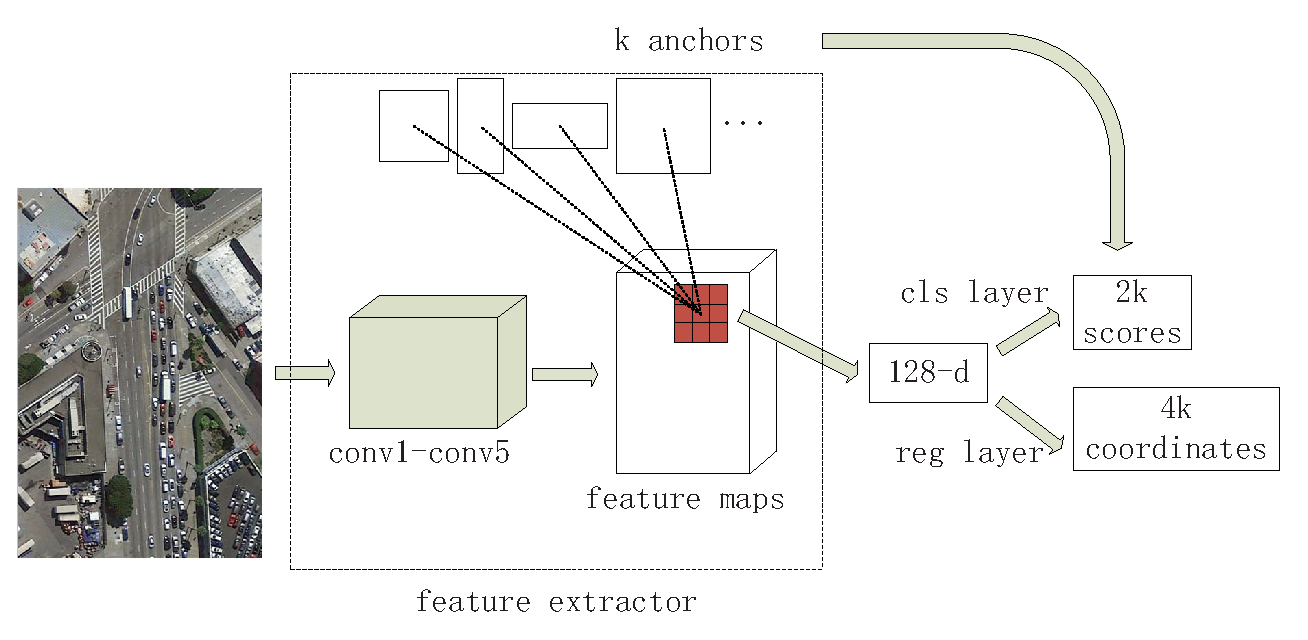
\includegraphics[height=5.0cm]{framework}
\caption{Our FCN-based detection framework. The input is a arbitrary-sized raw satellite image of 3 channels. A CNN of 5 convolution layers acts as a feature extractor. The two sibling parts, classification layer and regression layer do the following detection work. We use k anchors to hypothesize the vehicle locations}
\label{fig:example}
\end{figure}

\subsection{Architecture of FCN}

The architecture of FCN used in this paper is showed in figure 1. It consists of an feature extraction part and two sibling parts: classification and regression. In our experiments we investigate Zeiler and Fergus's model \cite{zfnet} which has 5 convolutional layers and 2 fully connected layers. ZF-net is designed for the ILSVRC classification competition \cite{ilsvrc} which has 1000 categories. As for detection task, it is not suitable for fully connected layers lose spatial information. So we replace the fully connected layers with convolutional layers, forming a single fully convolutional network. For clarity we demonstrate our FCN in table 1. The FCN model has six 3$\times$3 convolutional layers and 2 sibling 1$\times$1 convolutional layers. Every spatial position (corresponding to a region of the input image) of conv6 feature map obtains a 256-d feature vector, which is fed into the box-classification layer (cls.) and box-regression layer. Our model has the same depth with ZF-net but much less parameters. In practice, we compared our fully convolutional network model with ZF-net model and found that our model is 14 times smaller. 

\vspace{-3ex}

\setlength{\tabcolsep}{4pt}
\begin{table}
%\setlength{\abovecaptionskip}{-10pt}
%\setlength{\belowcaptionskip}{1pt}
\begin{center}
\caption{RPN configurations. For each convolutional layer ``parameters" gives the filter size and the stride which the filter is sliding with and ``filter numbers" gives the convolution kernel numbers of that layer. The pooling layers, LRN layers and ReLU activation layers are not shown for brevity}
\label{table:headings}
\begin{tabular}{ccccccccc}
\hline\noalign{\smallskip}
layer & conv1 & conv2 & conv3 & conv4 & conv5  & conv6 & cls & reg \\
\noalign{\smallskip}
\hline
\noalign{\smallskip}
parameters  &  3$\times$3,2  &  3$\times$3,2  &  3$\times$3,1  &  3$\times$3,1  &  3$\times$3,1  &  3$\times$3,1 &  1$\times$1,1 &  1$\times$1,1 \\
filter numbers & 96 & 256 & 384 & 384 & 256 & 256 & 18 & 36 \\
\hline
\end{tabular}
\end{center}
\end{table}
\setlength{\tabcolsep}{200pt}

%\vspace{-7ex}


\subsection{Learning methodology}
To narrow the vehicle object searching space, we use several reference windows (anchors \cite{faster-rcnn}) instead of searching every scale and aspect ratio. At training stage, our FCN model takes an arbitrary-sized image of 3 channels as input and generates feature maps of 256 channels after layer conv6. So in each position (x,y) of those features maps we can extract a 256-dimension vector corresponding to k anchors in the original image. If one anchor has intersection-over-union (IoU) overlap with any ground-truth box higher than 0.75 we take it as a positive sample and similarly, if the IoU is lower than 0.3 we consider it as a negative sample. Other reference boxes do not server as training examples. For anchors we use three 3 scales with boxes areas of 36$\times$36, 44$\times$44, and 50$\times$50 pixels, and 3 aspect ratios of 2:1,1:1, and 1:2. The 9 anchors we use are shown in table 2.

\vspace{-3ex}
\setlength{\tabcolsep}{4pt}
\begin{table}
\begin{center}
\caption{anchors }
\label{table:headings}
\begin{tabular}{ccccccccc}
\hline\noalign{\smallskip}
36$^{2}$,2:1 & 36$^{2}$,1:1 & 36$^{2}$,1:2 & 44$^{2}$,2:1 & 44$^{2}$,1:1 & 44$^{2}$,1:2 & 50$^{2}$,2:1 & 50$^{2}$,1:1 & 50$^{2}$,1:2\\
\noalign{\smallskip}
\hline
\noalign{\smallskip}
50$\times$26 & 36$\times$36 & 26$\times$50 & 62$\times$31 & 44$\times$44 & 31$\times$62 & 70$\times$36 & 50$\times$50 & 36$\times$70 \\
\hline
\end{tabular}
\end{center}
\end{table}
\setlength{\tabcolsep}{1.4pt}
\vspace{-5ex}

Our FCN model is trained end-to-end by back-propagation(BP)\cite{lecun89} and the optimization scheme we use is stochastic gradient descent(SGD)\cite{lecun89}. We define our multi-task loss function following \cite{fast-rcnn}:
\begin{equation}
  \L(\left\{p_{i}\right\},\left\{t_{i}\right\}) = \frac{1}{N_{cls}}\sum_{i}L_{cls}(p_{i},p_{i}^{*})+\lambda\frac{1}{N_{reg}}
  \sum_{i}p_{i}^{*}L_{reg}(t_{i},t_{i}^{*})\ . 
\end{equation}
 Here, i is the index of anchors in a mini-batch and p$_{i}$ is the predicted probability of anchor i being an object. The corresponding ground-truth label of p$_{i}$ is p$_{i}^{*}$ which is 1 if the anchor is positive and 0 otherwise. Similarly, t$_{i}$ is the 4 predicted parameterized coordinates of the predicted bounding box and t$_{i}^{*}$ the ground-truth. The classification loss L$_{cls}$ is a vehicle vs. non-vehicle log loss and we use smooth function defined in \cite{fast-rcnn} for regression loss L$_{reg}$. The hyperparameter $\lambda$ controls the balance between the two task losses. We find that satisfactory results can be obtained for vehicle detection by setting $\lambda$ = 10. Thus we keep this parameter fixed in the following experiments.Our implementation is based on Caffe\cite{caffe} and Python.




\section{Experiment}
This part dispatches details of our experiment results. Specificly, we first introduce our dataset and then we compare the detection accuracy of our method with that of some typical methods. Finally our method is compared to other DNN-based methods on the subject of size and speed.   
   
The dataset we use is that of \cite{xychen-hy} which includes 63 satellite images (1368$\times$972) from google earth of San Francisco city containing 6887 vehicle samples. To guarantee adequate training data, we split the dataset to 46 and 17 for training and testing randomly. At training stage, we augment the training set by rotating the images by 90$^{\circ}$, 180$^{\circ}$, 270$^{\circ}$ and flipping the images horizontally. No further data augmentation is done. When training, parameters of conv1-conv5 are initialized from a pre-trained model on PASCAL VOC2007 detection task. We iterate 10000 times with learning rate 0.001 for the first 7000 mini-batches and 0.0001 for the next 3000 mini-batches on our training set. The momentum and weight decay we use are 0.9 and 0.0005 respectively \cite{alexnet}.

Here the false alarm rate (FAR), precision rate (PR), and recall rate(RR) are defined as 


\begin{equation} 
\left\{
\begin{aligned}
FAR & = & \frac{number \ of \ false \ alarms}{number \ of \ vehicles} & \times 100 \% \\
PR  & = & \frac{number \ of \ detected \ vehicles}{number \ of \ detected \ objects} & \times 100 \% \\
RR  & = & \frac{number \ of \ detected \ vehicles}{number \ of \ vehicles}& \times 100 \%
\end{aligned}
\ .
\right.
\end{equation}

\setlength{\tabcolsep}{4pt}
\begin{table}% 加*表示跨栏,一般在双栏paper中使用
\begin{center}
\setlength{\abovecaptionskip}{-7pt}
\caption{FAR and processing time of our method and other methods on vehicle test set}
\label{table:headings}
{\begin{tabular}{|c|c|c|c|c|c|c|}% 列中文本左对齐,r:列中文本右对齐,c:列中文本居中
\hline
method & \multicolumn{6}{|c|}{FAR at given RR (\%)} \\
\cline{2-7}
 &\ 95\% & 90\% & 85\% & 80\% & 75\% & 70\% \\
\hline
Proposed & 22.3  & 11.8 & 7.38 & 4.88 & 3.41 & 2.54 \\
\hline
DNN & 23.5 & 12.2 & 7.5 & 5.07 & 3.45 & 2.61 \\
\hline
HOG+SVM\cite{hogsvm} & 67.5 & 43.4 & 29.3 & 20.2 & 14.3 & 10.3 \\
\hline
LBP+SVM\cite{lbpsvm} & 87.6  & 59.2 & 43.0 & 32.8 & 24.5 & 19.4 \\
\hline
Adaboost\cite{adaboost} & 91.6 & 65.3 & 49.1 & 40.1 & 31.6 & 25.8 \\
\hline
\multicolumn{7}{|c|}{test time for one image(s)} \\
\hline
\multicolumn{2}{|c|}{Proposed GPU} & \multicolumn{5}{|c|}{0.2}\\

\hline
\multicolumn{2}{|c|}{DNN\cite{xychen-hy} GPU} & \multicolumn{5}{|c|}{8}\\
\hline
\end{tabular}}
\end{center}
\end{table}

In table 3, We list the FAR at given RR of our method and 4 other typical methods. Our method outperforms other methods. It means our detector is more robust for it can detect objects which are very hard for the rest methods and that proves the benefits of deep convolutional features and position regression. In fig. 2, we give some detection results samples. The testing images cover scenes from road with many trees to parking lot. Our detector performs very well even vehicle objects are quite dense on parking pot or sheltered by trees.


\begin{figure}
\centering
\includegraphics[height=6.0cm]{results}
\caption{Some detection results in San Francisco. The four images cover scenes from road with trees to parking lot}
\label{fig:example}
\end{figure}


Since our detection framework is designed to be a single-stage detector, it also has a very fast speed. In table 3, we give the processing time of one image of FCN and traditional DNN method. Our detector achieves a frame rate of 5 fps on a computer with NVIDIA GTX960. There are two main reasons that our method is superior in speed. One is discarding proposal extraction stage which is an essential step of the rest methods and the other is that we do convolutions to the whole original image to extract features rather than one proposal by another. So for one testing image, our network does forward propagation only once while the other methods need to do it hundreds or thousands times depending on how many region proposals they extract in the region proposals extracting stage.

Table 4 shows the comparison of parameter size for various models. Our FCN model is based on ZF-Net but the size is only 1/14 of ZF-Net which demonstrates that using convolutional layers instead of fully connected layers can greatly reduce the the amount of model parameters while obtaining comparable detection performance.

\setlength{\tabcolsep}{4pt}
\begin{table}% 加*表示跨栏,一般在双栏paper中使用
\begin{center}
\setlength{\abovecaptionskip}{-7pt}
\caption{Size of parameters in various models}
\label{table:headings}
{\begin{tabular}{|c|c|c|c|}% 列中文本左对齐,r:列中文本右对齐,c:列中文本居中

\hline
Model & AlexNet \cite{alexnet}  & ZF-Net \cite{zfnet} & Proposed \\
\hline
size & 224MB & 249MB & 17MB  \\


\hline
\end{tabular}}
\end{center}
\end{table}

\section{Conclusion}
In this paper, we propose a new automatic satellite vehicle detection framework based on fully convolutional network (FCN). Different from traditional manual feature-based or DNN-based methods which are designed multi-stages, our method takes only one stage both in training and testing. By elaborating the FCN architecture and integrating several learning tricks, a very robust and real-time vehicle detector is obtained. Our experiment results show that our approach achieves better performance in both detection accuracy and speed in comparison to alternative approaches.

\bibliographystyle{splncs}
\bibliography{egbib}

\end{document}
